\documentclass[12pt]{article}
\setlength\parindent{0pt}
\usepackage[letterpaper, portrait, margin=1in]{geometry}
\usepackage{float}
\usepackage{graphicx}
\usepackage{listings}
\usepackage[]{indentfirst}
\usepackage{setspace}
\usepackage{amsmath}
\usepackage{fancyhdr}
\usepackage[nottoc,notlot,notlof]{tocbibind}
\pagestyle{fancy}
\lhead{Team \#1926141}
\rhead{Page \thepage \space of \pageref{LastPage}}
\usepackage{lastpage}
\doublespacing

\begin{document}

\begin{titlepage}

\newcommand{\HRule}{\rule{\linewidth}{0.5mm}}

\center
 
\textsc{\LARGE University of Colorado - Boulder}\\[1cm]
\textsc{\large COMAP ICM 2019}\\[0.5cm] % Major heading such as course name
\textsc{\large Problem D}\\[0.5cm] % Minor heading such as course title

\HRule \\[0.5cm]
{ \huge \bfseries Time to Leave the Louvre }\\[0.1cm] 
\HRule \\[.4cm]

\begin{figure}[H]
  \centering\includegraphics[width=.5\linewidth]{yeees.png}
  %\caption{}
  \label{fig:yeeees}
\end{figure}

\vfill
\begin{minipage}{0.4\textwidth}
\begin{flushleft} \large
\emph{Authors:}\\
William \textsc{Boshell} \\
Joel  
 \textsc{Courtney}
\end{flushleft}


\end{minipage}
~
\begin{minipage}{0.4\textwidth}
\begin{flushright} \large
\emph{Team ID:} \\
\textsc{1926141} 
\end{flushright}
\end{minipage}\\[1cm]


{\large \today}\\[1cm]
%\includegraphics[width=0.65\textwidth]{Titlepic.jpg}\\ 
 

\end{titlepage}
\newpage

\tableofcontents
\newpage

\section{Introduction}
As terror attacks become more common in France, reviewing evacuation routes at major public places is especially important. One such destination is the Mus\'ee de Louvre (Louvre Museum, or the Louvre for short) in Paris. It drew a world record 10.2 million visitors in 2018 [1], making it a prime target for an attack. In the event of such an attack, or any other situation requiring an immediate evacuation, people need to quickly head towards the optimal exit. Determining the optimal exit requires a model of the Louvre that captures the layout and exits. The model must also attempt to capture how people, including those with disabilities, behave and allow emergency personnel to reach the spots where the attacks occur. Finally, it also needs to account for potential secret exits, the quantity and locations of which are unknown for security purposes. 

\section{The Model}
\subsection{Motivation}
To determine escape routes, we first needed some sort of model of the Louvre that, at the very least, took into account rooms, stairs, elevators, and exits. We determined that a \textit{graph} would be the best way to do this. The basic definition of a graph is a set of \textit{nodes} that are connected by various \textit{edges}. Nodes can have wide range of properties depending on the implementation (see sections 2.2 and 2.3 for a discussion on the specific nodes used for this problem), but it is critical that each node has a unique identifier. On the other hand, edges simply connect 2 nodes using the aforementioned identifiers. They may or may not have an associated weight (e.g. distance between nodes) direction (for example, node 1 can be connected to node 2 without node 2 connecting to node 1, and occasionally other properties (depending on the problem). There are several different pathfinding methods (such as Dijkstra's algorithm) to navigate graphs. These methods are particularly useful for this problem, since an evacuation route is basically the shortest path to an exit.\\

We must also consider how people behave. The model needs to account for room capacity, door width (which controls how quickly people can enter and exit rooms), disabled people (who cannot use stairs or escalators), and emergency personnel (who go towards the situation as fast as possible). Capacity and door width are modeled as node properties. Disabled people and emergency personnel can be represented with special flags on a person object that interacts with the graph. These interactions are modeled through properties of the nodes. 

\subsection{Development}
The first step to developing the graph was to determine what types of nodes were needed and the properties of each type. Each type of node has a unique node ID and coordinates to indicate where in the museum they are.
\begin{itemize}
\item \textit{Room nodes} represent rooms and have an associated area, door width, and number. Area is roughly proportional to capacity, door width allows for flow, and number allows multiple rooms similar connected to each other to be modelled as one node rather than several as long as they are connected to at most 2 other rooms.
\item \textit{Stair nodes} represent stairs or escalators and connect to stair nodes on adjacent floors. They have an area (which is again used to determine capacity) and width, which is the number of people who can enter or exit at a time.
\item \textit{Elevator nodes} represent elevators and connect to other elevator nodes, which are not necessarily on adjacent floors. They also have a width, but no area since a fixed capacity is used instead.
\item \textit{Disabled lift nodes} function exactly the same as elevator nodes, except only disabled people can use them.
\item \textit{Exit nodes} only have a node ID and coordinates. They have infinite capacity since someone who reaches an exit node has left the building.
\end{itemize}

To get an accurate model of the Louvre, we first needed a detailed map [2] and other supplementary images [3],[4] when the map was unclear. The map was then loaded floor by floor into a node generator program we coded. This node generator allows the user to specify the node type, click 4 times around the edges of the node to get the area and center coordinates, enter the width (by clicking at each edge of a door for room nodes or estimating for stairs and elevators), and exit the program when done. The data generated from this process was written to a file upon exiting, and the complete list was made by combining these files. There are 474 total nodes.\\
Once the node locations were determined, they were plotted floor by floor as a visual aid for determining the edges. We used undirected edges since there would be a two way connection most of the time and realistic cases where they would be one way are covered by the pathfinding algorithm. Edges between floors were added by carefully examining where the stairs and elevators lined up on the maps of adjacent floors. There are 569 total edges.

\subsection{Implementation}
%Please do this. Discuss the types of people, nuances of stairs and elevators (incl. disabled lifts), room flow, capacity, groups, pathfinding (how you ran Dijkstra's at the very beginning of the simulation and gave the people their routes), directions in the nodes, anything else you can think of related to this. I consider finding the nodes and edges development of the model and everything else done with the graph implementation.

\subsubsection{Graph Construction}
The model is implemented in three large steps. First, the node and edges lists are converted into a basic undirected, cyclic graph which contains only the information needed for the simulation (data such as the coordinates of the corners of each node is discarded because it is only needed for plotting the results, for example.). The nodes of the basic graph contain all of the information about the Louvre, but have no behavior (rooms cannot hold people yet, elevators don't move, etc).\\

Next, the conditions of the simulation are imposed. A few nodes are marked as Dangerous, and edges can be deleted to block the flow of traffic and force people to find another route. Once the conditions are set, the paths for each kind of person is pre-computed using Dijkstra's algorithm. Two Single Source Shortest Path trees (SSSP) are made from each exit; the first is able to traverse stairs but not allowed to use lifts reserved for disabled people, and the second is allowed to use all lifts, but not able to move on stairs. A third set of SSSP trees is then computed from the dangerous nodes so that emergency personel can find their way to the source, rather than away from it. The SSSP trees of each type are then compared at each node to find the paths to the closest exit and the closest emergency. The full SSSP trees are then discarded.\\

We chose to pre-compute the paths instead of letting the people do their own pathfinding for two reasons. First, allowing thousands of people to rerun Dijkstra's algorithm every time their path needed to change would be very costly, and not worth the added computation time. The simulation already takes on the order of a minute for some starting conditions, but redoing Dijkstra's algorithm every time a path is blocked would likely make the simulation infeasible to run. Second, it would be unrealistic to give every person knowledge of the layout of the whole building. Most people will rely on exit signs posted at junctions for directions.\\

The last step is to convert the basic graph into the full graph which runs the simulation. Each node is converted to actual \textit{Room}, \textit{Elevator}, \textit{Stair}, \textit{Exit}, and \textit{Dangerous Room} objects which have their own behavior. The edges are converted to pairs of directed \textit{Passages}. Each Passage contains a reference to the opposite node, and each pair of Passages share a reference to a \textit{Door} object which keeps count of how many people have crossed the edge in either direction. Each node contains a list of each Passage its connected to, as well as the pathfinding information indicating which Passage is the ideal path.\\

A limitation of manually creating the nodes and edges list is that tracing out the full detail of each room would be too time-consuming; to simplify this, entire blocks of exhibits were marked as a single node, with a parameter indicating how many actual rooms it contained. We account for this during the graph construction by adding in extra Rooms as needed, splitting the Rooms on either side of the node they came from. In the output from the simulation, these extra Rooms are recombined with the node they came from, to simplify the rendering process. The graph is now ready to be populated before the simulation is run.

\subsubsection{Adding People}
In the control, approximately 9000 total people are added to the graph ($\pm20$ people depending on randomly generated group sizes). The majority of people are normal Tourists, while about $1\%$ of people in groups are disabled, and about $1\%$ of people not in groups are emergency personnel. About $20\%$ of all Tourists are alone [4, p. 14], and the rest are in groups of sizes ranging from 2 to 15, with an extra bias toward groups of size 2 to 5 (to approximate the number of families). In the control, everyone is placed randomly throughout the building with no bias toward more popular rooms. All members of groups start in the same room. Once everyone has been added to the graph, the simulation is ready to begin.

\subsubsection{Room Behavior}
Each Door in the simulation counts the number of people that has passed through it in either direction, and after a certain number it stops "allowing" people through (which simulates too many people trying to move through the same door at a time). This counter is reset after every update tick.\\

Each room has two behaviors associated with it: what to do on each update tick, and how to "decide" if it can allow more people into the room.
\begin{itemize}
    \item \textit{Rooms}: Normal rooms have a maximum capacity based on the physical area traced out on the map; if they reach that capacity, no more people will fit in the room until someone leaves. On each update tick, each person in the room tries to move too the next room in their path, if possible.
    \item \textit{Exits}: Exits have infinite capacity, and movement to an exit is only limited by the Door that precedes it. On each update tick, each person in the exit is removed from the simulation entirely.
    \item \textit{Stairs}: Stairs have a minimum wait time and a maximum capacity. It must be under-capacity for someone to enter, and once on the stairs they must wait a set number of ticks before they can leave (this simulates the time it takes to traverse stairs and escalators).
    \item \textit{Elevators}: Elevators behave similarly to Stairs, except they only allow entry and exit at certain times. (This simulates the doors closing, and the process of letting people exit before anyone else can enter.)
    \item \textit{Disabled Lifts}: Disabled lifts behave the same as elevators, but will be excluded from the pathfinding for people without physical disabilities during the graph construction.
\end{itemize}

\subsubsection{People and Group Behavior}
Different Person types only differ in the pathfinding decisions they make; Tourists follow the path to the exits without using Disabled Lifts, Disabled Tourist follow the path to the exits without using Stairs, and Emergency Personnel follow the path to the closest Dangerous Room. But, with several thousand people trying to take similar routes or opposite routes, this inevitably leads to bottlenecks and stalemates (where the people in two adjacent at-capacity rooms are trying to pass each other). Stalemates are not very realistic (and cause the simulation to never finish), so too combat this, each person has a small chance to try a suboptimal path upon finding that the next room is full.\\

Groups are still modelled as individual people, but they share a group ID. Their movement behaviors are unchanged, but in order to keep the group together, they indirectly affect the movement of people around them. For a short time after a member of a group walks through a door, only other members of the same group will be able to follow them. The chances that someone else can follow increases by $10\%$ each time someone tries to do so. This is slightly unrealistic in that the effect persists after the entire group has moved to the next room; but it does a good job keeping groups together in most cases, and allowing groups to be broken up if enough people try to force their way in.

\section{Results and Analysis}
\subsection{Control Test} %xbar=5319, sigma=621
For the control test, we simulated 250 runs with 9000 people in the museum, no secret exits, and a stair wait time (how long it takes people to go up or down a flight of stairs or an escalator) of 5 ticks. The number of people was determined by taking the product of number of visitors (10,200,000) and average visit length (2 hours and 42 minutes, which is exactly 2.7 hours [4, p. 14]) for a total of 27,540,000 person-hours and dividing it by the number of hours per year the museum is open per year (57.5 hours per week [2, p. 3] times $\frac{365}{7}$ weeks per year, for a total of about 2,998 hours per year). This comes out to an average of about 9,185 people in the museum at a time. Obviously, this will be more or less at certain times, but this gives a reasonable baseline for our control test. The results are shown in Figure 1:
\begin{figure}[H]
	\centering
	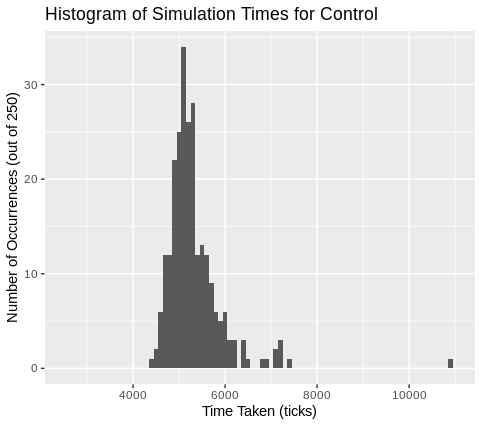
\includegraphics[width=5in]{control.png}
    \caption{Histogram of control test.}
\end{figure}
Note that simulation time is the number of ticks it takes until the last person exits the museum. This shows a roughly normal distribution skewed slightly to the right, a smaller peak further to the right, and an extreme outlier. The sample mean was $\Bar{x}=5319$ and the sample variance was $s=613$.

\subsection{Sensitivity Analysis}
After analyzing the control data, we could then do sensitivity analysis by separately varying each of the 3 major parameters.
\subsubsection{Number of People}
The first parameter we varied was the number of people, n, initially in the Louvre. 581 simulations were run for various n and the results are shown in Figure 2:
\begin{figure}[H]
	\centering
	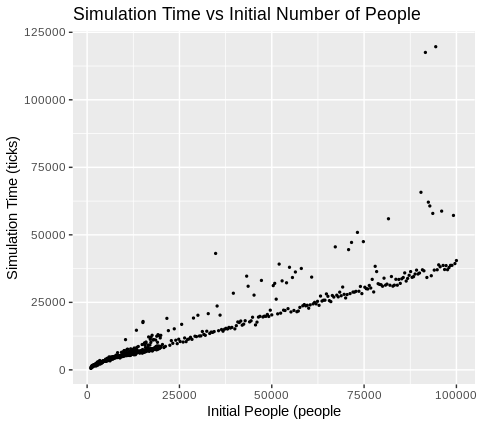
\includegraphics[width=5in]{vspeople.png}
    \caption{Plot of sensitivity to number of people.}
\end{figure}
For large n ($\geq 10,000$ or so), this shows that the time to fully evacuate the Louvre is linear in n. This is expected since the exits can only accommodate a finite number of people at a time. Because of this, there are always bottlenecks near the exits for large. This is also expected since thousands of people heading towards 4 exits should bottleneck. However, there are 2 different slopes for the lines. This is unexpected, but can be explained by considering that it would scale differently depending on whether every exit is saturated. If not, then the simulation time would scale at the lower rate. This appears to be the case most of the time. The exit that is only saturated some of the time is the Carrosuel du Louvre entrance in the second basement. This makes sense because the adjacent hallway is relatively large, pyramid reception area is enormous (almost $10\%$ of the total area in our model), and a relatively small number of people head towards it.\\

For small n, the simulation time increases with n, but slower than linearly. This makes sense because people could get caught in smaller bottlenecks in the museum (this gets more likely as n increases), but do not have to wait near exits for a long time.

\subsubsection{Stair Travel Time}
Next we changed the parameters of the nodes, such as elevator and stair capacity, and stair travel time. Most changes to the parameters did effectively nothing, but the simulation time varied highly with the time it takes to use the stairs. The relationship is shown below.

\begin{figure}[H]
	\centering
	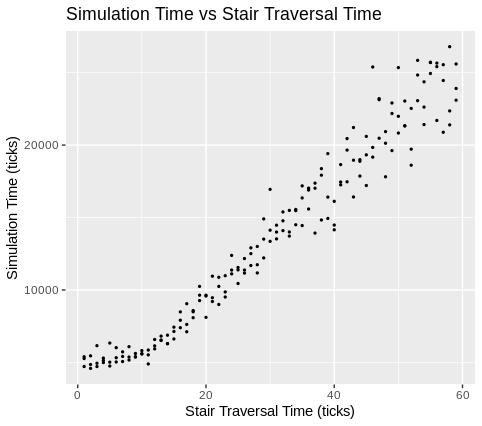
\includegraphics[width=5in]{vswait.png}
    \caption{Plot of sensitivity to stair travel time.}
\end{figure}

The high end of the travel time is somewhat unrealistic, but this clearly shows that the time it takes to change floors dominates. The slight concave up curve around $t_{travel} = 10$ shows that for low values, the time spent travelling between rooms dominates. But, as people spend more time on the stairs, they become crowded and turn into a bottleneck.

\subsubsection{Room Distribution Bias}
In an effort to make the starting conditions slightly more realistic, we added a bias toward placing people in the most popular rooms (such as the Mona Lisa exhibit). We did this with a bias $N$; giving each tourist and group a $1$ in $N$ chance to start in one of the top $15$ most popular rooms (otherwise, they would be randomly placed). The relationship between the bias and the simulation time is shown below.

\begin{figure}[H]
	\centering
	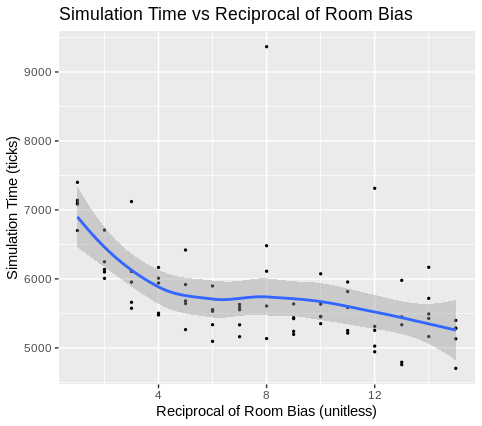
\includegraphics[width=5in]{vsbias.png}
    \caption{Plot of sensitivity to room distribution bias.}
\end{figure}

Realistic numbers for this distribution are likely between 1 in 5 and 1 in 10, so this distribution only starts to matter noticeably toward the extremely dense side around 1 in 5 to 1 in 4. This is likely because the redistribution is mostly just moving the bottlenecks around, not making them much worse.

\section{Strengths and Weaknesses of Model}
\subsection{Strengths}
The simulation is highly adjustable and general; the structure of the graph can be changed to fit the scenario depending on where the incident occurs, and which exits are available. This makes performing several randomized trials very simple. It is also a general model to all buildings. With proper floor plans, the model could simulate the Pentagon just as easily - the only requirement is that the building does not contain any rooms or structures other than the five main node types.\\

Our simulation is detailed and produces full time-lapsed video showing the evacuation process. It models the entire building down to the scale of individual rooms, people, and doorways. While it could still be made more accurate, it could not feasibly be more detailed.

\subsection{Weaknesses}
The simulation is in many ways a black box; it is very difficult to discern what is going on inside without rendering the result or breaking a lot of the object-oriented design to get concise diagnostic data that wouldn't otherwise be accessible. This can lead to situations where the simulation appears to run perfectly, but never terminates. The efficiency of the pathfinding is highly dependent on proper connection of the nodes, so any mistakes in the creation of the graph could cause strange, unrealistic behaviors that take a lot of time to track down.\\

The pathfinding method is very rigid; on a properly constructed graph it will always produce the right paths, but minor mistakes can make paths highly inefficient. For example, a person in Port des Lions should be able to move straight to the exit nearby; but when making the graph, we accidentally missed two edges that forced everyone to move up two floors, over to Denon wing, then down four floors into the Pyramid.\\

The parameters for stairs and elevators are estimates which are difficult to judge. The time it takes for an elevator to move between floors is dependent on the height of the floor and the speed of the elevator, and the time necessary to use the stairs is dependent on the height of the stairs and the people on it. And, since the simulation time scaled so highly with the stair traversal time parameter, if our estimates are wrong, the entire simulation is thrown off.\\

Lastly, and perhaps most importantly, our simulation does not perform well when modelling language barriers and differences in communication ability. We attempted multiple times to model foreign language speakers by having some people occasionally make wrong turns (presumably because they misread a sign, or misinterpreted someone's directions), but all changes in that area resulted in vast increases to the simulation time. Even if $1\%$ of the people make a wrong decision $1\%$ of the time, the simulation would say that it took days to evacuate everyone. This is obviously incorrect, and indicates that either our approach to the language barrier was misguided, or there are deep problems with the rest of the model that go unnoticed until it is introduced.

\section{Future Improvements and Conclusions}
%How technology improve routes, etc.
The most important improvements to our model could be made to the behavior of stairs and elevators, and the inclusion of communication difficulties. While the model is flexible and general, it is rarely straightforward to make fundamental changes to the behavior of the people and graph; and its ease of use is lacking.\\

If the more interesting predictions of our model is correct, then the evacuation time is steeply linearly dependent on how quickly people can move on stairs, and linearly dependent on the number of people at the museum. They shouldn't need to worry about the distribution of people around the exhibits, or with spacing out large tour groups.

\newpage
\begin{thebibliography}{1}

\bibitem{} Benaiteau, Marion. “10.2 Million Visitors to the Louvre in 2018.” Louvre, 3 Jan. 2019, presse.louvre.fr/10-2-million-visitors-to-the-louvre-in-2018/. 

\bibitem{} “Louvre-Plan-Visitors-Mobility-Impairments.pdf.” Louvre, www.louvre.fr/sites/default/files/medias/\\medias\_fichiers/fichiers/pdf/louvre-plan-visitors-mobility-impairments.pdf.

\bibitem{} Google Maps. Google, https://www.google.com/maps/@48.8612731,2.334932,456m/\\data=!3m1!1e3?hl=en

\bibitem{} Cuny, Christine. “‘Pyramid’ Project Launch.” Louvre, 18 Sept. 2014, www.louvre.fr/sites/default/files/dp\_pyramide 28102014\_en.pdf. 

\end{thebibliography}

\end{document}
